\documentclass{article}
\usepackage[utf8]{inputenc}
\usepackage{polyglossia}
\usepackage{amssymb,amsmath,amsthm}
\usepackage{bussproofs}
\usepackage{enumitem}
\usepackage{fontspec}
\setdefaultlanguage{russian}
\setotherlanguage{english}
\usepackage{translator}
\uselanguage{russian}
\languagepath{russian}
\setmainfont[Ligatures={TeX,Historic}]{CMU Serif}
\setsansfont{CMU Sans Serif}                    %% задаёт шрифт без засечек
\setmonofont{CMU Typewriter Text}               %% задаёт моноширинный шрифт
\usepackage[a4paper, margin=0.5cm]{geometry}
\usepackage{listings}
\usepackage{graphicx}
\pagenumbering{gobble}
%opening
\title{}
\author{}

\begin{document}

%\maketitle
%https://www.youtube.com/playlist?list=PLlb7e2G7aSpS634rDf15afbmKJRSYmH50

\section*{Measurements cheat sheet}

Этот листочек для измерения времени работы одной и той же программы на одном и том же датасете. Примеры будут на языке Python, чтобы инструкцию смогло осилить как можно больше народу. Некоторые моменты сильно упрощены, но для студенческих работ это ОК. В курсе матстатистики вам расскажут, как оно на самом деле работает.

\begin {enumerate}

\item Подготовьте тестовый стенд: отключите обновления, сбросьте все кэши, отключите фоновую музыку, закройте браузеры, стабилизируйте частоту CPU (например, выставьте на минимальную; если выставить на максимальную, CPU начнет перегреваться) etc. Проверьте алгоритм, входные данные, средство измерения на адекватность. Проконсультируйтесь с научным руководителем.

\item Проведите серию измерений. Желательно, чтобы количество замеров было больше 20 (ну, например, 40), но и не слишком большое: десятки тысяч измерений тоже довольно бестолково. Получите список значений:
\begin{lstlisting}[language=Python]
	t = (X1, X2, X3, ... Xn)
\end{lstlisting}

\item Подготовьтесь к анализу:
\begin{lstlisting}[language=Python]
	from scipy import stats
	import numpy as np
	import matplotlib.pyplot as plt
\end{lstlisting}

\item Изучите, как распределены данные. Постройте гистограмму, посмотрите на нее. На гистограмме не должно быть сильных выбросов. Если выброс одиночный, то его можно отбросить\footnote{Методологически надо применить формальные критерии (напр., Шовене), но мы упростим себе жизнь и просто отбросим.}. Но только если он один! Если их несколько, то см пункт 1.
\begin{lstlisting}[language=Python]
	plt.hist(t)
\end{lstlisting}

\begin{figure}[h]
\centering
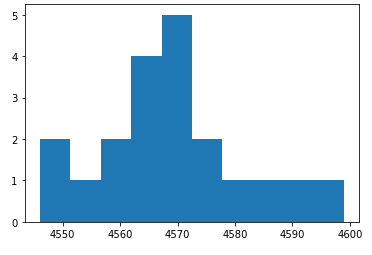
\includegraphics[height=4cm]{hist.png}
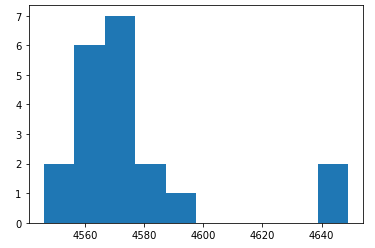
\includegraphics[height=4cm]{hist2.png}
\caption{Пример <<хорошей>> (слева) и <<плохой>> (справа) гистограмм}
\end{figure}

\item Проверьте, что данные проходят некоторые тесты на нормальность. В нашем случае признаком успешного прохождения теста является p-value $> 0.05$ хотя бы на одном тесте. Если тесты не проходятся, см пункт 1.
\begin{lstlisting}[language=Python]
	stats.normaltest(t)
	stats.shapiro(t)
\end{lstlisting}

\item Вычислите среднее и стандартное отклонение. Стандартное отклонение не должно быть слишком большим ($5-10\%$ от среднего). Если оно большое, см пункт 1.
\begin{lstlisting}[language=Python]
	np.mean(t)
	np.std(t, ddof=1)
\end{lstlisting}

\item Определите, нужен ли вам доверительный интервал. Если да, то вычислите его. В примере используется уровень доверия $95\%$:
\begin{lstlisting}[language=Python]
	stats.t.ppf(0.975, df=len(t)-1)*stats.sem(t)
\end{lstlisting}
Примечание: 0.975 --- это не опечатка.

\item Определите, какая именно случайная погрешность вам нужна, затем сложите полученную случайную погрешность с погрешностью инструмента измерения.

\item Проведите округление в соответствии с принятыми правилами. Не нужно выносить на слайды те числа, которые напечатал скрипт:
$$ \text{Погрешность}: 12.879372652772872 \rightarrow 13 $$
$$ \text{Среднее}: 4568.8 \rightarrow 4569 $$
$$ \text{Интервал записывается так}: 4569 \pm 13 $$
\begin{itemize}
\item В погрешности оставьте одну значащую цифру (или две, если первая значащая цифра единица)
\item Среднее округлите до той точности, с которой приведена погрешность.
\end{itemize}

\item Если у вас много разных величин разных порядков, имеет смысл вычислять относительные погрешности вместо абсолютных. Так нагляднее.
\end{enumerate}

\end{document}
